\documentclass[journal]{IEEEtran}

\usepackage[usenames,dvipsnames,svgnames,table]{xcolor}
\usepackage{amsmath}
\usepackage{amsfonts}
\usepackage{cite}
\usepackage{graphicx}
\usepackage{listings}
\usepackage{multirow}
\usepackage{tabularx}
\usepackage{varioref}
\usepackage{hyperref}
\usepackage[noabbrev,capitalize]{cleveref}
\usepackage[group-separator={,}, group-four-digits=true]{siunitx}
\usepackage{lscape}
\usepackage{bm}
\usepackage{chngpage}
\usepackage{blindtext} % For filler text

\usepackage[english]{babel}
\usepackage[utf8]{inputenc}

%Includes "References" in the table of contents
\usepackage[nottoc]{tocbibind}


\lstset{
  frame=single,
  basicstyle=\ttfamily,% print whole listing small
  language=R,
  aboveskip=3mm,
  belowskip=3mm,
  showstringspaces=false,
  columns=flexible,
  numbers=none,
  commentstyle=\color{ForestGreen},
  stringstyle=\color{Maroon},
  breaklines=true,
  breakatwhitespace=true,
  tabsize=2,
  literate={<-}{{$\gets$}}1 {~}{{$\sim$}}1
}

\hypersetup{
  colorlinks=true,
  linkcolor=blue,
  urlcolor=blue,
}

\sisetup{output-exponent-marker=\textsc{e}}

\begin{document}

\title{Facial Keypoints Detection}
\author{Will Clark and Matthew DeLio\\
University of Chicago Booth School of Business\\
\textsf{\{will.clark,mdelio\}@chicagobooth.edu}}

% The paper headers
\markboth{Machine Learning (BUS 41201) Final Project}
{Machine Learning (BUS 41204) Final Project}

\maketitle

\section{Summary}

\section{Modelling}
\subsection{Facial Keypoints Introduction}
\subsection{Building a Model (Tools \& Software)}


\subsection{Initial Models}
What we tried in a nutshell:
\begin{enumerate}
\item 3-level - 1 convolutional, 2 dense
\item 6-level - 3 convolutional, 3 dense
\item 6-level with dropout
\item Batch-size changes - size positively correlated with minimum loss-floor.
\item Varying learning rate/momentum: static, and dynamic (as prescribed by \cite{lasagnenesterov} to balance increasing momentum must decrease learning rate)
\item Wider layers
\item More/Less Dropout
\item Image Preprocessing
\item Amputated w/RF
\end{enumerate}

\subsection{Individual Feature Models}
Should outline how we came up with the idea of training different models for each feature (set of features).


Dropout, l1/l2 regularization, and momentum/learning rate.


Using the advice given in Andrew Ng's paper on regularization \cite{ng2004feature}, by acknowledging the fact that we have a dimensionally large input data-set, we choose to apply L1 regularization. <Talk about how we do see a more gradual, but smoother drop in the loss function>

Should plot some validation loss (rmse).

Include any citations for the blog we ran across with \cite{dnouri}

\subsection{Missing Feature Model}
Since the data contain many missing features caused by partially obscured images, our resulting model must also predict the presence of features.  To predict this we turn to a slightly modified version with a sigmoid non-linearity on the output layer and the binary cross-entropy loss function defined in \cref{eq:bin_cross}.

\[\label{eq:bin_cross}
 L = -target \log(p) - (1 - target) \log(1 - p)
\]
where \texttt{target} indicates whether the feature is actually missing ($\in \{0,1\}$) and \texttt{p} is the predicted probability of the feature being missing

For many of the features, the neural network does a good job separating the two classes and producing probabilities that make logical sense.  The ones that it doesn't separate well, like \texttt{Left Eye Center}, \texttt{Right Eye Center} and \texttt{Mouth Center Bottom Lip}, have few missing data-point exemplars in the training data (9, 9, and 23 respectively out of 4934 samples).

\begin{figure}[!ht]
  \centering
  \caption{Boxplots for Missing Eye Features}
  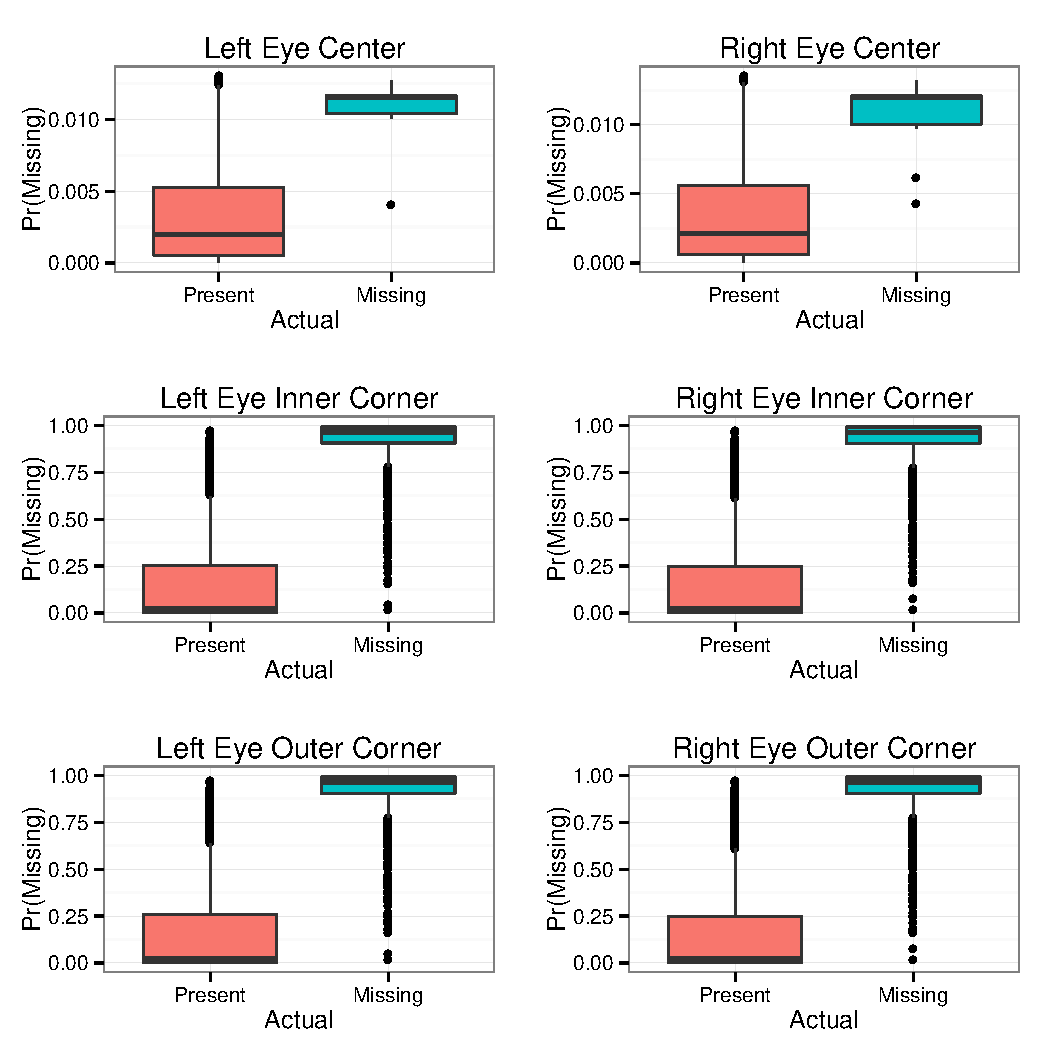
\includegraphics[scale=.5]{logistic_boxplots_eye.pdf}
  \label{fig:logistic_boxplots_eye}
\end{figure}

% We can probably drop these next two, they don't add much to the discussion...maybe we can just mention they they look identical (throw them in an appendix)
\begin{figure}[!ht]
  \centering
  \caption{Boxplots for Missing Eyebrow Features}
  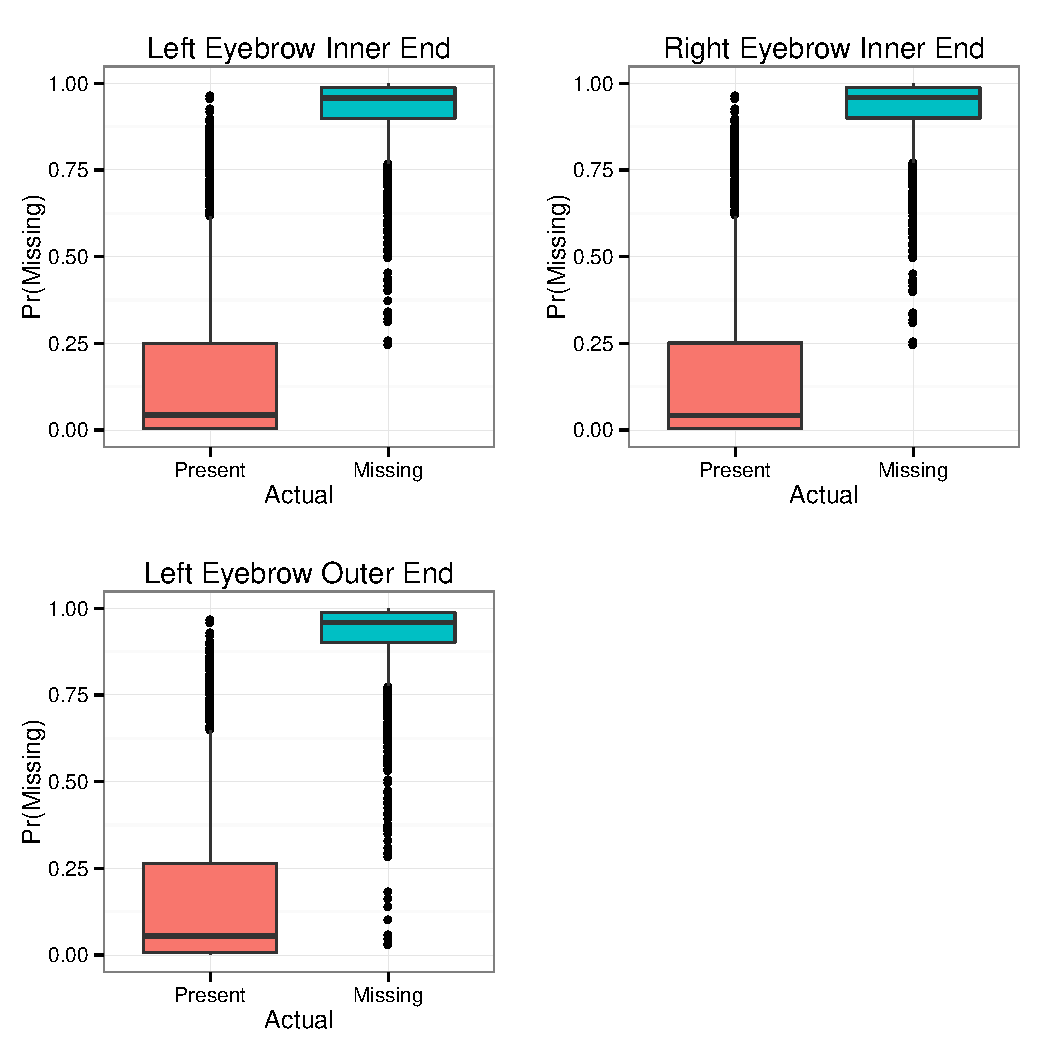
\includegraphics[scale=.5]{logistic_boxplots_eyebrow.pdf}
  \label{fig:logistic_boxplots_eyebrow}
\end{figure}

\begin{figure}[!ht]
  \centering
  \caption{Boxplots for Missing Mouth Features}
  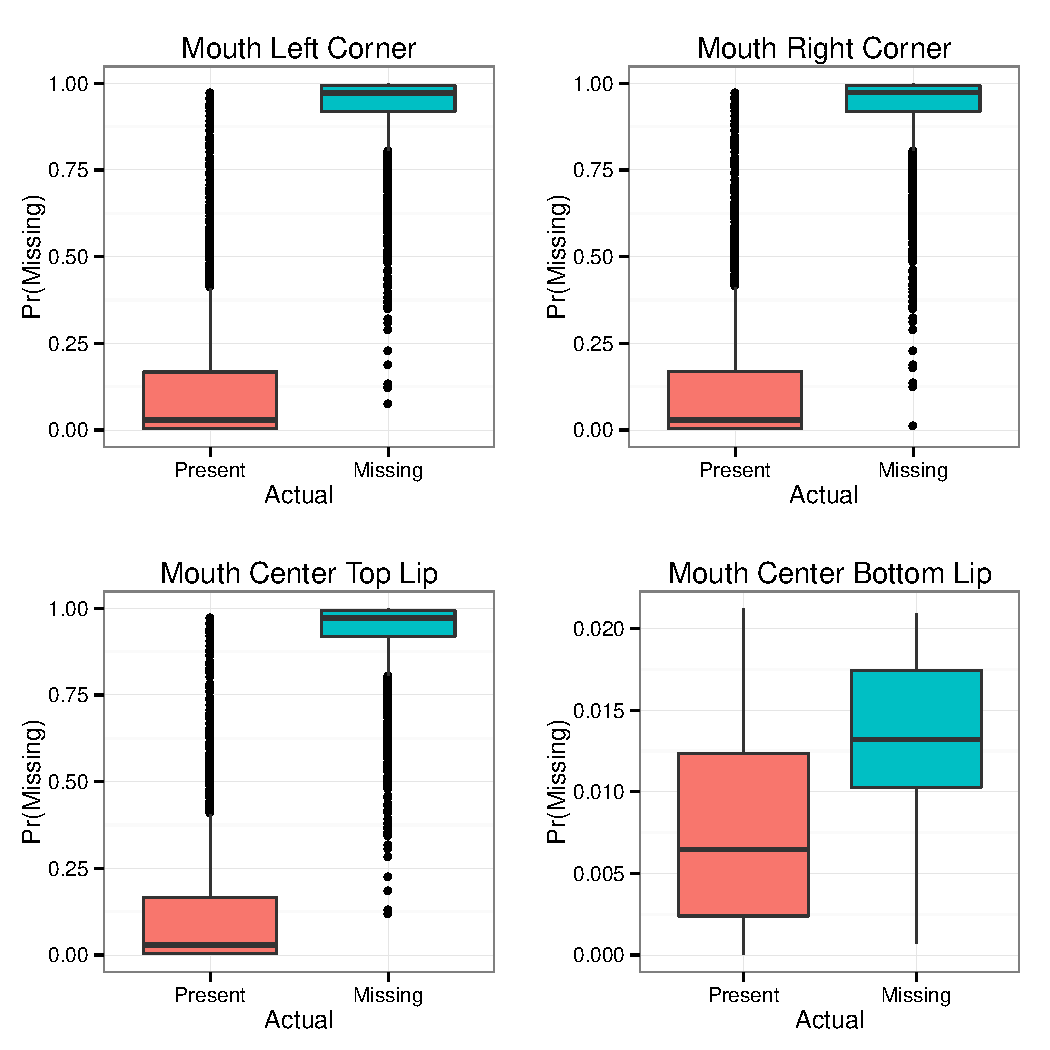
\includegraphics[scale=.5]{logistic_boxplots_mouth.pdf}
  \label{fig:logistic_boxplots_mouth}
\end{figure}

% \begin{figure}[!ht]
%   \centering
%   \caption{Boxplots for Missing Nose Feature}
%   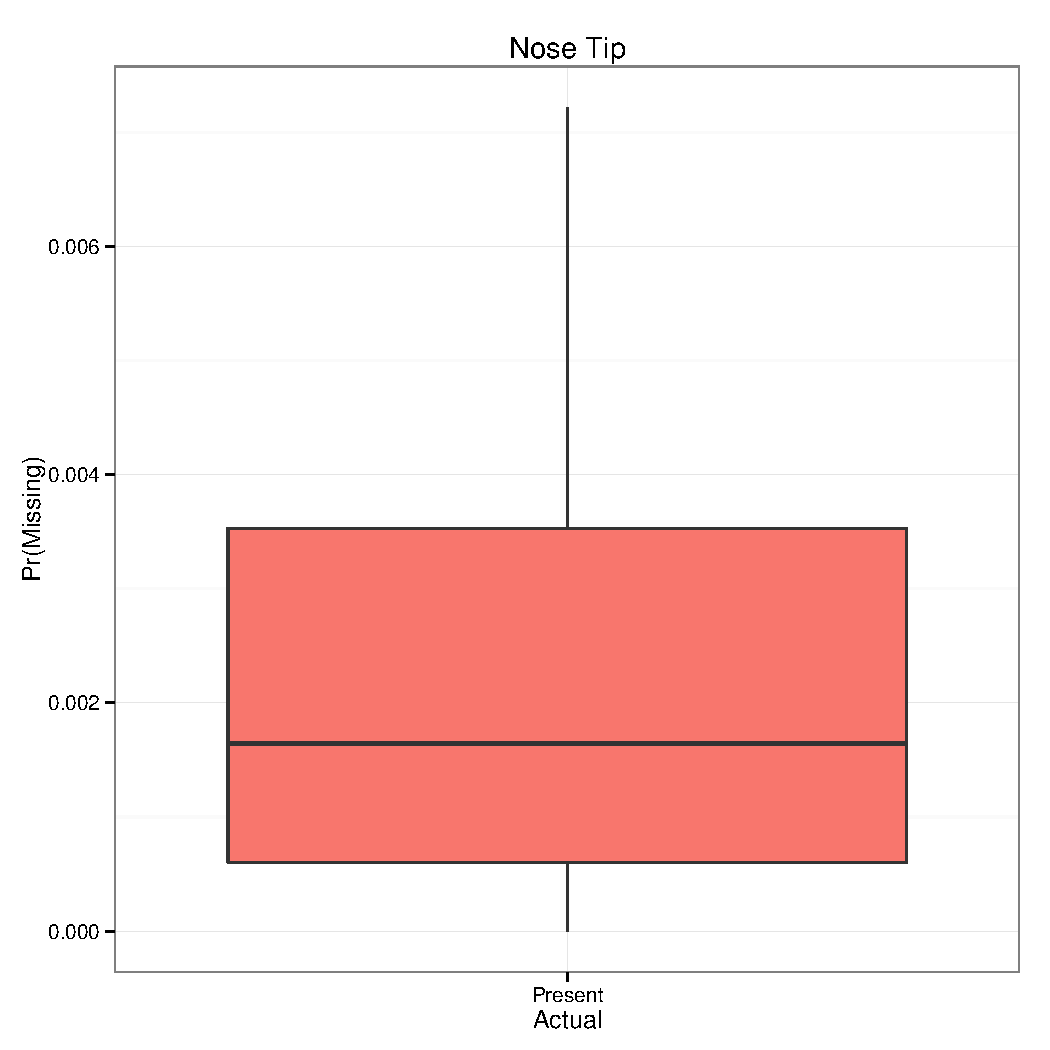
\includegraphics[scale=.5]{logistic_boxplots_nose.pdf}
%   \label{fig:logistic_boxplots_nose}
% \end{figure}

With the output trained, we next turn to determining the optimal cutoff.  Using the R package \texttt{OptimalCutpoints} we choose to maximize the accuracy area \cite{lewis2008use,greiner1995two,greiner1996two} which is defined in \cref{eq:roc_aa}.

\[\label{eq:roc_aa}
AA(c)=\frac{TP(c)TN(c)}{(TP(c)+FN(c))(FP(c)+TN(c))}
\]
where $TP$ = True Positives, $TN$ = True Negatives, $FN$ = False Negatives, \& $FP$ = False Positives

Looking over our boxplots, we see there are generally two categories of features: those that are missing often and those that are not.  For the ones that are missing often, we have a relatively good separability between the predicted probabilities.  For those that are not, the separately is questionable at best.  Turning to the ROC plot for a feature that is missing quite often, \texttt{Left Eye Inner Corner}, (see \cref{fig:roc_left_eye_inner_corner}) we see there is a lot of area under the ROC curve and the optimal cutoff point of 0.5 seems to put us right on the upper-left edge of the curve.  Next, looking at \texttt{Left Eye Center}, a feature with few missing exemplars, (see \cref{fig:roc_left_eye_center}) we see less area and a clear trade-off between specificity and sensitivity.  Again, a value of 0.5 seems to put us on the upper-left edge of the curve.

It turns out that, given the optimization condition, the best cutoff for all of these features is 0.5 (see \cref{tab:logistic_cutoff_table}\footnote{Note: that the \texttt{Nose Tip} feature is present in all training and validation images.}).  In each of the cases, we end up with quite a large sensitivity and a reasonable specificity.

\begin{figure}[!htb]
  \centering
  \caption{ROC Curve for Left Eye Inner Corner}
  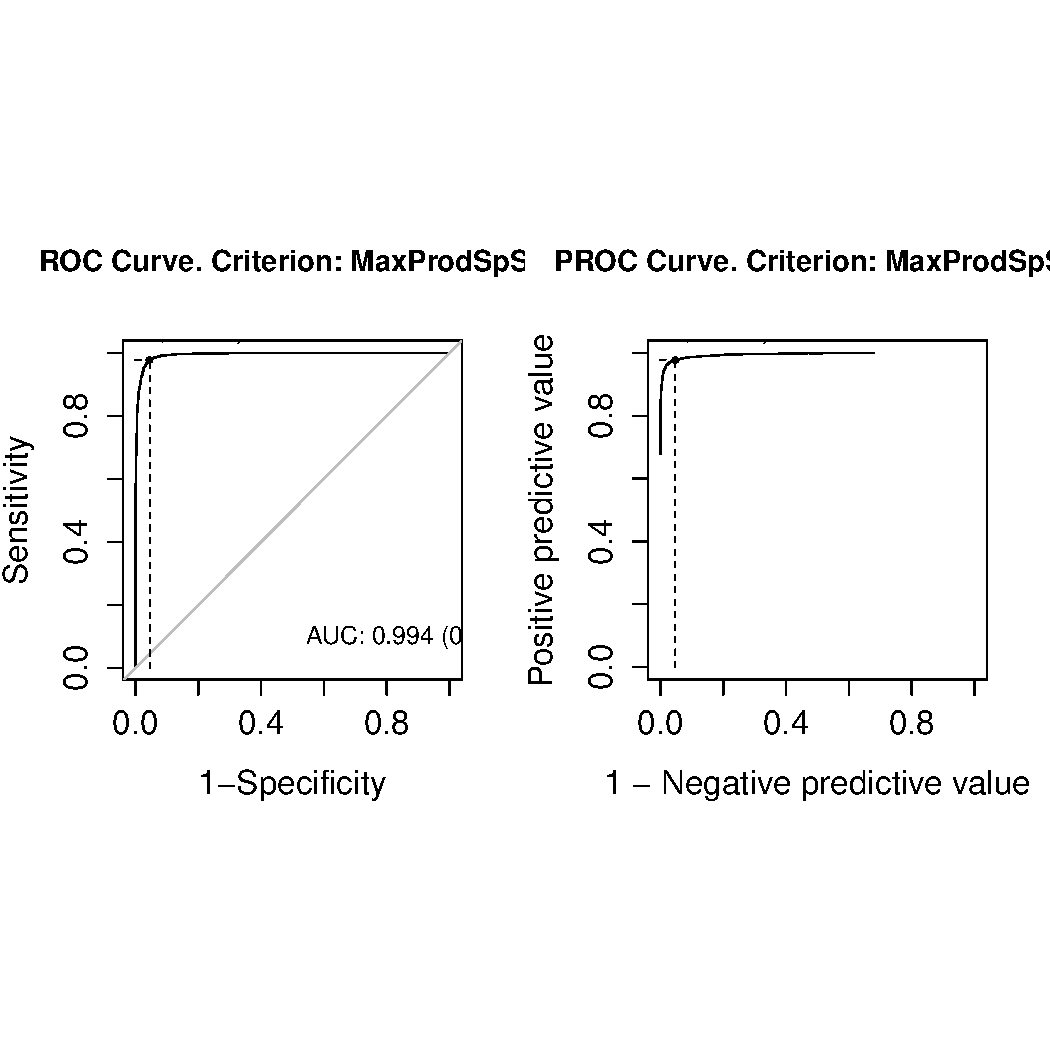
\includegraphics[scale=.5]{roc_left_eye_inner_corner.pdf}
  \label{fig:roc_left_eye_inner_corner}
\end{figure}

\begin{figure}[!htb]
  \centering
  \caption{ROC Curve For Left Eye Center Feature}
  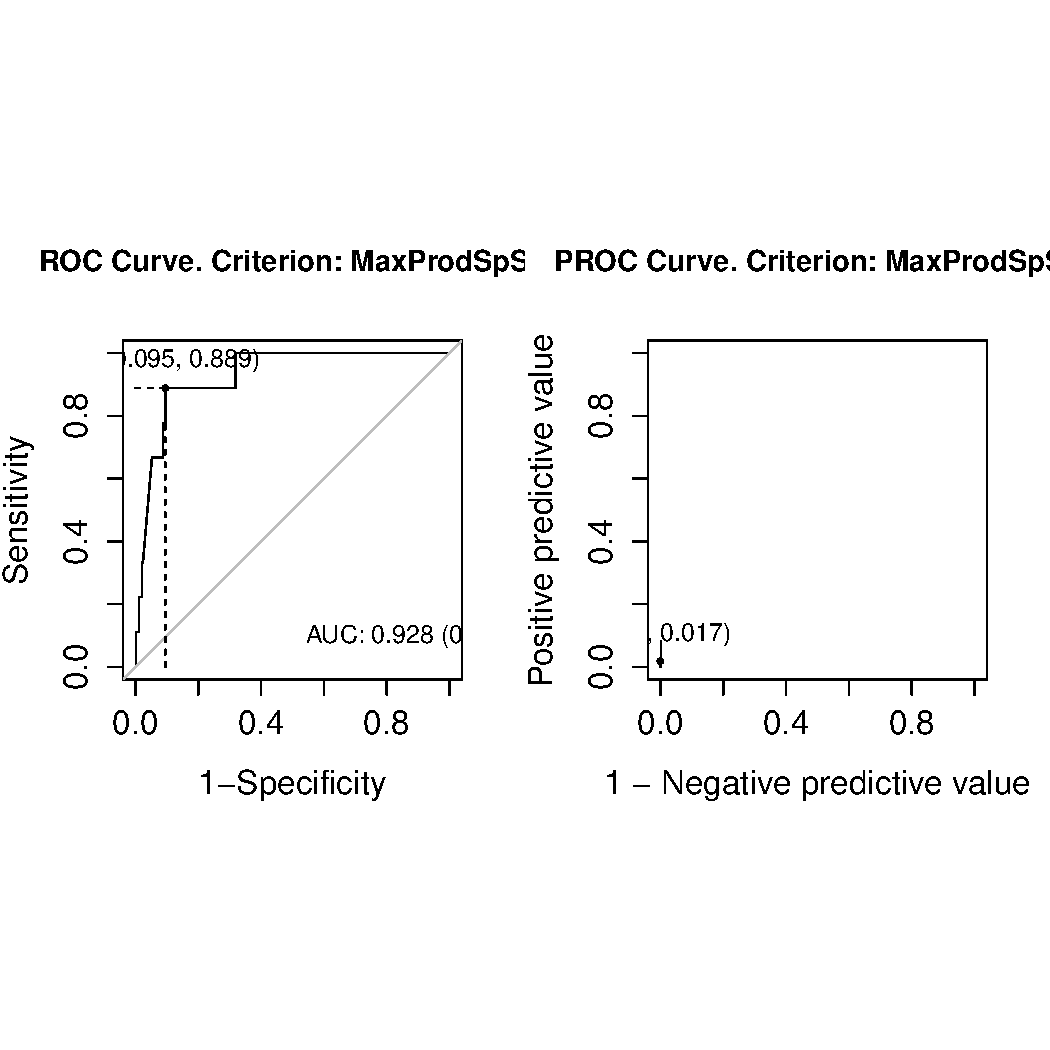
\includegraphics[scale=.5]{roc_left_eye_center.pdf}
  \label{fig:roc_left_eye_center}
\end{figure}


% latex table generated in R 3.2.2 by xtable 1.7-4 package
% Wed Dec  9 11:55:32 2015
\begin{table}[ht]
\centering
\caption{Cutoff Validation Performance} 
\label{tab:logistic_cutoff_table}
\begin{tabular}{lrrr}
  \hline
Feature & Cutoff & Sensitivity & Specificity \\ 
  \hline
Left Eye Center & 0.500 & 0.000 & 1.000 \\ 
  Right Eye Center & 0.500 & 0.000 & 1.000 \\ 
  Left Eye Inner Corner & 0.500 & 0.961 & 0.714 \\ 
  Right Eye Inner Corner & 0.500 & 0.962 & 0.715 \\ 
  Left Eye Outer Corner & 0.500 & 0.960 & 0.713 \\ 
  Right Eye Outer Corner & 0.500 & 0.961 & 0.715 \\ 
  Left Eyebrow Inner End & 0.500 & 0.961 & 0.714 \\ 
  Right Eyebrow Inner End & 0.500 & 0.961 & 0.716 \\ 
  Left Eyebrow Outer End & 0.500 & 0.963 & 0.713 \\ 
  Right Eyebrow Outer End & 0.500 & 0.963 & 0.720 \\ 
  Nose Tip & 0.500 &  &  \\ 
  Mouth Left Corner & 0.500 & 0.961 & 0.718 \\ 
  Mouth Right Corner & 0.500 & 0.960 & 0.716 \\ 
  Mouth Center Top Lip & 0.500 & 0.960 & 0.717 \\ 
  Mouth Center Bottom Lip & 0.500 & 0.000 & 1.000 \\ 
   \hline
\end{tabular}
\end{table}


\subsection{Combined Loss Model}
Semi-failed attempt to train missing signals and coordinates simultaneously.
\subsection{Putting It All Together}
Show examples

\section{Kaggle Submission}
Ranking?

\section{Applications}
\begin{enumerate}
\item Engagement Detection
\end{enumerate}

\medskip

\bibliographystyle{IEEEtran}
% \bibliographystyle{unsrt}
\bibliography{citations}

\end{document}

% \input{.tex}

% \begin{figure}[!htb]
%   \centering
%   \begin{subfigure}[b]{0.49\textwidth}
%     \caption{}
%     \includegraphics[width=\textwidth]{.pdf}
%     \label{fig:}
%   \end{subfigure}
%   \hfill
%   \begin{subfigure}[b]{0.49\textwidth}
%     \caption{}
%     \includegraphics[width=\textwidth]{.pdf}
%     \label{fig:}
%   \end{subfigure}
%   \caption{}
% \end{figure}

% \begin{figure}[!htb]
%   \centering
%   \caption{}
%   \includegraphics[scale=.5]{.pdf}
%   \label{fig:}
% \end{figure}